\chapter{Introduction}
\label{chap:introduction}

\section{Contexte et Problématique}
\label{sec:contexte}

La modélisation du trafic routier est devenue un outil essentiel pour la planification et la gestion des infrastructures de transport dans le monde entier. Cependant, les modèles traditionnels, développés principalement dans le contexte des pays industrialisés, se heurtent à des limites importantes lorsqu'ils sont appliqués aux réalités des pays en développement, et particulièrement au Bénin.

\subsection{Importance de la Modélisation du Trafic}
\label{subsec:importance}

La modélisation du trafic routier offre plusieurs avantages fondamentaux pour le développement et la gestion des infrastructures :

\begin{itemize}
\item Elle permet d'\textbf{anticiper les congestions} et d'optimiser les flux de véhicules;
\item Elle constitue un \textbf{outil d'aide à la décision} pour les investissements routiers;
\item Elle facilite l'\textbf{évaluation des impacts} environnementaux et économiques des politiques de transport;
\item Elle contribue à l'\textbf{amélioration de la sécurité routière} par l'identification des points critiques du réseau.
\end{itemize}

Dans un contexte de croissance urbaine rapide comme celui du Bénin, ces outils deviennent particulièrement précieux pour accompagner un développement durable des infrastructures.

\subsection{Défis Spécifiques au Bénin}
\label{subsec:defis_benin}

Le réseau routier béninois présente des particularités qui rendent inadéquate l'application directe des modèles classiques de trafic :

\begin{itemize}
\item \textbf{Hétérogénéité marquée du trafic} : coexistence de véhicules aux caractéristiques très différentes (voitures, camions, bus, et surtout motos);
\item \textbf{Prédominance des motos} (localement appelées Zémidjans lorsqu'elles servent de taxi), représentant plus de 70\% du parc automobile, avec des comportements de conduite spécifiques;
\item \textbf{Diversité des infrastructures routières} : routes bitumées, en terre, pavées, pistes informelles, souvent en état de dégradation variable;
\item \textbf{Comportements de conduite adaptés aux contraintes locales}, notamment les pratiques de gap-filling et d'interweaving des motos;
\item \textbf{Réglementation routière appliquée de manière variable} et présence importante de négociations informelles aux intersections.
\end{itemize}

\begin{figure}[htbp]
\centering
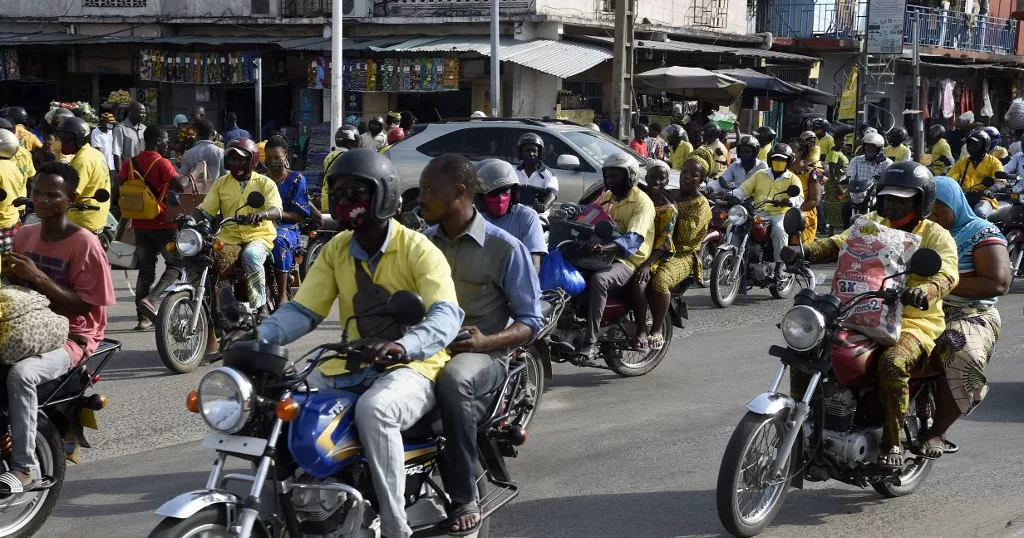
\includegraphics[width=0.8\textwidth]{images/introduction/trafic_cotonou}
\caption{Trafic typique à Cotonou montrant la prédominance des motos (Zémidjans) et leur comportement spécifique dans la circulation.}
\label{fig:trafic_cotonou}
\end{figure}

\subsection{Limites des Modèles Classiques}
\label{subsec:limites_modeles}

Le modèle LWR (Lighthill-Whitham-Richards), largement utilisé pour la modélisation macroscopique du trafic, repose sur plusieurs hypothèses qui s'avèrent inadaptées au contexte béninois :

\begin{itemize}
\item \textbf{Homogénéité des véhicules} : le modèle standard suppose une flotte uniforme, ce qui est très éloigné de la réalité béninoise;
\item \textbf{Relation vitesse-densité unique} : cette relation ne tient pas compte des différences de comportement entre classes de véhicules;
\item \textbf{Impact du revêtement routier négligé} : la qualité variable des routes influence pourtant significativement la dynamique du trafic;
\item \textbf{Absence de modélisation des comportements spécifiques} comme le gap-filling des motos;
\item \textbf{Traitement inadéquat des intersections} qui constituent des points névralgiques dans le réseau béninois.
\end{itemize}

Face à ces limites, il devient nécessaire de développer une extension du modèle LWR spécifiquement adaptée au contexte béninois.

\section{Objectifs de l'Étude}
\label{sec:objectifs}

Cette recherche vise à développer un modèle macroscopique de trafic routier adapté aux spécificités du Bénin, en poursuivant les objectifs suivants :

\begin{enumerate}
\item \textbf{Adapter le modèle LWR au contexte béninois} en préservant sa robustesse mathématique et sa simplicité relative;
\item \textbf{Intégrer la diversité des classes de véhicules}, avec une attention particulière aux motos et à leur comportement spécifique;
\item \textbf{Prendre en compte l'impact des infrastructures routières} sur la dynamique du trafic, notamment la qualité variable du revêtement;
\item \textbf{Modéliser efficacement les intersections} et autres singularités du réseau routier béninois;
\item \textbf{Développer un outil opérationnel} pour la planification et la gestion du trafic routier au Bénin;
\item \textbf{Valider le modèle avec des données locales} collectées sur le terrain.
\end{enumerate}

Ces objectifs s'inscrivent dans une démarche plus large visant à améliorer la compréhension et la gestion des systèmes de transport dans les pays en développement, en tenant compte de leurs spécificités.

\section{Contributions de l'Étude}
\label{sec:contributions}

Cette étude apporte plusieurs contributions significatives à la modélisation du trafic routier :

\subsection{Contributions Théoriques}
\label{subsec:contrib_theoriques}

\begin{itemize}
\item \textbf{Extension multiclasses du modèle LWR} intégrant des équations de conservation couplées pour chaque type de véhicule;
\item \textbf{Introduction d'un coefficient de ralentissement} $\lambda_{\text{mat},i}$ lié au revêtement routier pour chaque classe de véhicule;
\item \textbf{Développement de fonctions de modulation} $f_{M,i}(\rho_M)$ pour représenter l'influence des motos sur les autres classes de véhicules;
\item \textbf{Formalisation mathématique} des phénomènes de gap-filling et d'interweaving observés dans le trafic béninois.
\end{itemize}

\subsection{Contributions Méthodologiques et Pratiques}
\label{subsec:contrib_pratiques}

\begin{itemize}
\item \textbf{Méthodes de calibration spécifiques} pour les paramètres du modèle à partir de données réelles du Bénin;
\item \textbf{Techniques de validation adaptées} au contexte des pays en développement, où les données peuvent être parcellaires;
\item \textbf{Analyses de sensibilité quantitatives} permettant d'identifier les paramètres les plus influents du modèle;
\item \textbf{Cadre d'application opérationnel} pour l'utilisation du modèle dans la planification des infrastructures au Bénin.
\end{itemize}

Ces contributions visent à combler un vide important dans la littérature scientifique, où les modèles de trafic sont rarement adaptés aux spécificités des pays en développement, et particulièrement à la prévalence des deux-roues motorisés.

\section{Structure du Document}
\label{sec:structure}

Pour présenter notre travail de manière claire et structurée, ce document est organisé comme suit :

\begin{itemize}
\item Le \textbf{Chapitre \ref{chap:fondements_theoriques}} présente les fondements théoriques du modèle LWR standard, ses équations, ses propriétés mathématiques et ses limites.

\item Le \textbf{Chapitre \ref{chap:specificites_benin}} analyse en détail les spécificités du réseau routier béninois et le rôle particulier des motos dans la dynamique du trafic local.

\item Le \textbf{Chapitre \ref{chap:extension_modele}} développe notre extension du modèle LWR, avec l'approche multiclasses, les fonctions de modulation pour les motos, et le coefficient de ralentissement lié au revêtement.

\item Le \textbf{Chapitre \ref{chap:calibrage_validation}} présente les méthodes et résultats de calibration et de validation du modèle à partir de données collectées sur le terrain au Bénin.

\item Le \textbf{Chapitre \ref{chap:analyse_sensibilite}} propose une analyse de sensibilité des paramètres du modèle pour évaluer leur impact relatif sur les prédictions.

\item Le \textbf{Chapitre \ref{chap:intersections}} approfondit la modélisation des intersections et des changements de voie, points critiques du réseau béninois.

\item Le \textbf{Chapitre \ref{chap:aspects_stochastiques}} intègre des aspects stochastiques et comportementaux pour améliorer la précision du modèle.

\item Le \textbf{Chapitre \ref{chap:discussion}} discute les forces et limites du modèle proposé et envisage des perspectives d'amélioration.

\item Le \textbf{Chapitre \ref{chap:conclusion}} synthétise les principales contributions et conclut sur l'importance d'adapter les modèles de trafic aux contextes spécifiques des pays en développement.
\end{itemize}

Cette structure progressive permet d'aborder le problème depuis ses fondements théoriques jusqu'aux applications pratiques, en mettant en lumière la spécificité du contexte béninois et les innovations apportées par notre extension du modèle LWR.
